\section{論文作成の例}

\verb|\section{論文作成の例}|と書くと上のように表示される.

\subsection{図表挿入の例}

\verb|\subsection{図表挿入の例}|と書くと上のように表示される.

\subsubsection{表の例}

\verb|\subsubsection{表の例}|と書くと上のように表示される.表\ref{tab:restaurant}は表の例である.

\begin{table}[htb]
\caption{食欲を満たす方法と特徴.}
\label{tab:restaurant}
\begin{center}
\begin{tabular}{c|c|c}\hline\hline
 & 値段 & スピード \\\hline
高級料亭 & 高い & 遅い  \\
ファミリーレストラン & 中ぐらい & 中ぐらい  \\
ファーストフード & 安い & 早い \\
\hline\hline
\end{tabular}
\end{center}
\end{table}

\begin{figure}[h]
\centering
\includegraphics%[scale=0.5]
[width=5cm]{wissfig_.eps} 
\caption{図面の例}
\label{figure:one_image}
\end{figure} 

\subsubsection*{図の例}

\verb|\subsubsection*{図の例}|と書くと上のように表示される.アスタリスク
(*)をつけたことにより番号が表示されない.図\ref{figure:one_image}は論文
中に図面を挿入した例である.

\subsection*{図表の配置}
全ての図表は「…を図 5に示す」「…である(表 2).」というように本文から引用し,図表自体はその文と同じページか,それ以降のページに配置する.読む順番の観点から,初出の文章より前のページに図を掲載することは厳禁である.

まれに,編集中に図の位置がずれてヘッダやフッタ部に重なってしまっていることがあるので,投稿前に十分に確認されたい.

\begin{figure*}[ht]
\centering
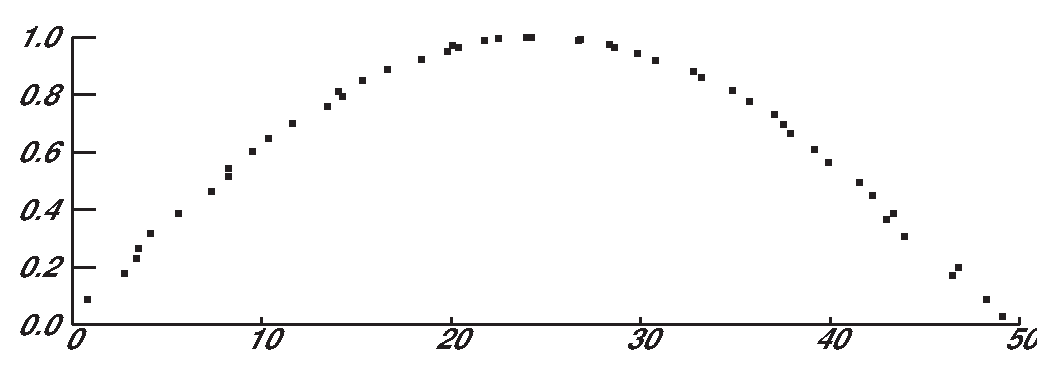
\includegraphics[scale=0.6]{graph_.eps} 
\caption{グラフの例}
\label{figure:graph}
\end{figure*} 

図\ref{figure:graph}は,2段抜きの図の例である.2段抜きの図を挿入するとき
には,\verb|\begin{figure}|の代わりに\verb|\begin{figure*}|とし,
\verb|\end{figure*}|で終わるようにすればよい.同様に\verb|table|について
も\verb|*|をつけることで2段抜きにできる.

ただし2段抜きの図や表は,\LaTeX によって別のページに移動して張り付けられ
てしまうことが多いので注意が必要である.

\subsection{キャプション,図表中のテキスト}
図表のキャプションについては,図の場合は図の下,表の場合は表の上に配置する.

図中の注釈などのテキストはキャプションと同じかやや小さいサイズ,読みやすさの観点ではゴシック系フォントの利用が望ましい.表のテキストもキャプションと同じかやや小さいサイズが望ましい.

\subsection{図作成上の注意点}
原稿を作成する場合,著者は必ず仕上がりを確認し,図が鮮明に,意図した場所に出
力されることを確認する.特に,次の点に留意すること.
\begin{itemize}

 \item 画面キャプチャした画像を使って図を作る際,非可逆圧縮を使わないこ
       と.画面キャプチャした画像をファイルに保存する場合には,保存形式
       として非圧縮形式(BMP等)または可逆圧縮形式(GIF,PNG等) を用いる.

 \item 図に文字を使って注釈を書き込む場合,極力,アウトラインデータの文
       字を用いること.ビットマップデータの文字を用いた場合,文字の輪郭
       がギザギザに見える.
\end{itemize}

\subsection{数式の例}
数式の書き方の詳細はIEEE style manual\cite{IEEE2014}を参照.長すぎる数式は適宜改行し,余白にはみ出さないようにすること.

式(\ref{eqn:sum})は数式の例である.

\begin{equation}
\sum^{N}_{n=1}n = \frac{1}{2}N(N+1)
\label{eqn:sum}
\end{equation}

\subsection{節と項の数について}
1つの章の中に節を作るときは必ず複数個の節を作ること.1個しか節を作る必要がないときはそもそも節に分ける必要がない,ということである.同様に,1節の中に1個しか項がない,という場合も章構成を見直す.

良い例)1章→1.1節,1.2節,2章…

悪い例)1章→1.1節,2章…